\documentclass[9pt,twocolumn,twoside,lineno]{gsag3jnl}

\articletype{inv} % article type
% {inv} Investigations
% {msr} Mutant Screen Reports
% {gs} Genomic Selection
% {goi} Genetics of Immunity 
% {gos} Genetics of Sex 
% {mp} Multiparental Populations

\title{Real Time Genome Scan Using GPU}

\author[$\ast$]{Xiaoqi Hu}
\author[$\ast$]{Hyeonju Kim}
\author[$\ast$]{Saunak Sen}

\affil[$\ast$]{University of Tennessee Health Science Center}

\keywords{Linear Model \\ Genome Scan \\ GPU}

\runningtitle{G3 Journal Template on Overleaf} % For use in the footer 

%% For the footnote.
%% Give the last name of the first author if only one author;
% \runningauthor{FirstAuthorLastname}
%% last names of both authors if there are two authors;
% \runningauthor{FirstAuthorLastname and SecondAuthorLastname}
%% last name of the first author followed by et al, if more than two authors.
\runningauthor{Hu \textit{et al.}}

\begin{abstract}
The BXD strains are an important reference population of
recombinant inbred lines which have been phenotyped extensively.
To facilitate interactive use of genotype-phenotype relationships
in this population, we sought to speed up eQTL scans where we
perform a univariate genome scan for every trait in a collection
of omic traits.  By using easily parallelizable operations such as
matrix multiplication, vectorized operations, and elementwise
operations, we are able to decrease runtimes approaching real-time
computation.  We used parallelization using different CPU threads
as well as GPUs.  We found that the speed advantage of GPUs is
dependent on problem size and shape.  These results indicate a pathway for
speeding up eQTL scans using LMMs.  Our implementation is in the
Julia programming language.

\end{abstract}

\begin{document}

\maketitle
\thispagestyle{firststyle}
\logomark
\articletypemark
\marginmark
\firstpagefootnote

% Use the \equalcontrib command to mark authors with equal
% contributions, using the relevant superscript numbers
\equalcontrib{1}
\equalcontrib{2}

\correspondingauthoraffiliation{3}{Corresponding author: Please insert the affiliation correspondence address and email for the corresponding author. The corresponding author should be marked with the relevant number in the author list, as shown in the example.}
\vspace{-34pt}% Only used for adjusting extra space in the left column of the first page

\noindent        Computational demands in omics are growing exponentially. For
instance, eQTL analysis requires processing genomewide
expression and marker data; this can take minutes, hours or
days depending on problem size.  Scientists want to intereact
with the results and real-time processing would be valuable.
Our goal is to build a backend for GeneNetwork that will enable
real-time genome scans for important genetic reference
populations such as the BXD population.


\section{Methods and Data}
\label{sec:methods:Data}

%Manuscripts submitted to G3 should contain a clear description of the experimental design in sufficient detail so that the experimental analysis could be repeated by another scientist. If the level of detail necessary to explain the protocol goes beyond two paragraphs, give a short description in the main body of the paper and prepare a detailed description for supporting information.  For example, details would include indicating how many individuals were used, and if applicable how individuals or groups were combined for analysis. If working with mutants indicate how many independent mutants were isolated. If working with populations indicate how samples were collected and whether they were random with respect to the target population.

\subsection{Linear Model} 
 Let $y_i$ denote a vector of gene expressions for $n$
individuals in the $i$-th omics trait ( $i=1,\ldots,m$).  We
define a univariate linear model as follows:

\begin{eqnarray*}
	y_i &=& X_j \beta_j+ \epsilon_i,
	\quad \epsilon_i \sim N(0,\sigma_i^2)
\end{eqnarray*}

where ${X}_j$ is a matrix that may include the $y-$intercept with
or without covariate(s), and the $j$-th candidate genetic marker
($j=1,\ldots,p$).  ${\beta}_j$ is a vector of the $j$-th eQTL
effects, and ${\epsilon}_i$ is random error.  Suppose $RSS_{0i}$
is a residual sum of squares under the null hypothesis of no eQTL
and $RSS_{1ij}$ is the residual sum of squares under the
alternative for the $i$-th trait and $j$-th marker.  Then the LOD
score for the corresponding pair can be written as:

\begin{eqnarray*}
	LOD_{ij} &=& \frac{n}{2} \log_{10} \left( \frac{RSS_{0i}}{RSS_{1ij}} \right)\\
	&=& \frac{n}{2} \log_{10} \left( 1{-}r_{ij}^2 \right),
\end{eqnarray*}
where $r_{ij}$ is the correlation between the $i$-th trait and
$j$-th marker. Note that this only works for one-df tests.  If the
trait matrix and genotype matrix ($G$) are standardized, then the
correlation matrix is simply $$R=Y^{'}G.$$
%Indicate which statistical analysis has been performed and describe the method and model applied. If many genes were examined simultaneously, or many phenotypes, a multiple comparison correction should be used to control the type I error rate, or a rationale for not applying a correction must be provided. The type of correction applied should be clearly stated. It should also be clear whether the p-values reported are raw, or after correction. Corrected p-values are often appropriate, but raw p-values should be available in the supporting materials so that others may perform their own corrections. 

\subsection{Acceleration Techniques}
We used various techniques to accelerate eQTL scans. 
\subsubsection{Multithreaded CPU operations}
 Used for multi-threaded loops whenever possible, eg. for element-wise operations
\subsubsection{Matrix and Vectorized Operations}
 OpenBLAS for multi-threaded matrix operations. 
Matrix multiplication is a well studied area where the computer scientists try to apply various optimization techniques to make it run faster. 
There are various BLAS libraries available, such as gslBLAS, OpenBLAS, etc. 
The matrix multiplication in OpenBLAS is default multithreaded, therefore does not require extra coding effort to achieve highly efficient result. 
 
\subsubsection{Single precision}
 Faster and memory efficient; may be less accurate, but acceptable for quick scan
Most dataset used in scientific computing are stored in double precision. 


\subsubsection{GPU operations}
Specialized computations such as matrix multiplications and element-wise operations; requires additional programming effort
\subsubsection{Julia language}
Programming simplicity of interpreted languages with speed approaching compiled languages; GPU programming and linear algebra straightforward
\subsubsection{ Heritability grid}
For LMMs, considering a discrete grid of heritabilities enhances parallelization


\subsection{Information and Availability of Datasets}
Data from 79 BXD strains for 35556 transcripts from spleens were collected using the Affy Mouse Gene 1.0 ST array. Animals were generated by Drs. Lu, Williams, and colleagues. There were usu- ally one male and one female per strain; strain averages were used as the trait of analysis. All animals were young adults (oldest 160 days). GN accession: GN283. Marker data was available on 7321 markers; genotype probabilities were calculated using R/qtl.

      \begin{figure}[!htb]

	\caption{Schematic of data and correlation calculation: $Y$ is
		the expression phenotype matrix, $G$ is the matrix of
		genotytpes, and $R=Y^{\prime}G$ is the matrix of
		correlations.  The LOD scores are a function of the
		correlation matrix.}
	\label{MatrixMult}
	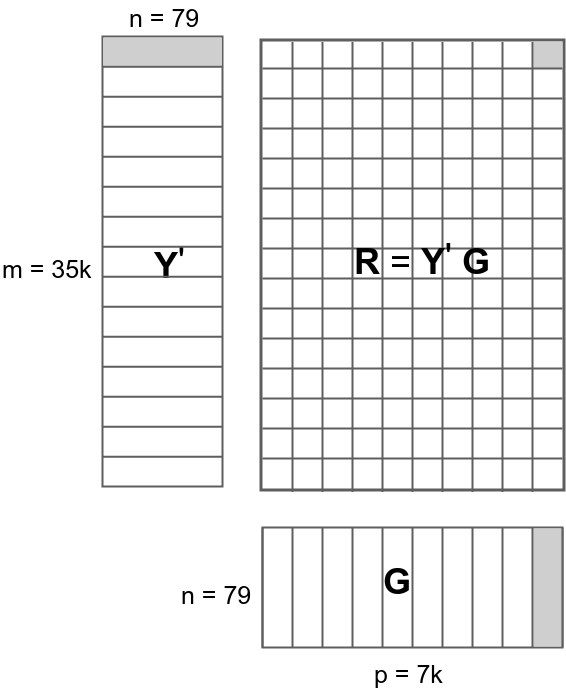
\includegraphics[scale = .4]{figs/YGmatrix.png}
\end{figure}    

%At the end of the Materials and Methods section, include a statement on reagent and data availability. Please read the Data and Reagent Policy before writing the statement. Make sure to list the accession numbers or DOIs of any data you have placed in public repositories. List the file names and descriptions of any data you will upload as supplemental information. The statement should also include any applicable IRB numbers. You may include specifications for how to properly acknowledge or cite the data.

%For example: Strains are available upon request. File S1 contains detailed descriptions of all supplemental files. File S2 contains SNP ID numbers and locations. File S3 contains genotypes for each individual. Sequence data are available at GenBank and the accession numbers are listed in File S3. Gene expression data are available at GEO with the accession number: GDS1234. Code used to generate the simulated data is provided in file S4. 

\section{Results}
{\em Profiling:} Calculating correlation matrix and LOD score
takes up to 90\% of runtime.  Both involve matrix operations
(multiplication and elementwise operations respectively) which
are highly parallelizable.
      \begin{itemize}
	\item We chose OpenBLAS library for matrix multiplication, an
	optimized multithreaded library.  In our experiment, gslBLAS
	(GNU Scientific Library) is 10 times slower than OpenBLAS.
	\item We used multithreading operations whenever possible, such as
	for elementwise operations.
	\item We explored using single precision instead of double
	precision.  Precision change affects both throughput (FLOPS) and
	data transfer time.  Single precision is twice
	as fast as double precision, and provides correct result
	within 1e-2 tolerance (Table 1).
\end{itemize}

 {\em GPUs vs CPUs:} GPUs are attractive since they provide a
massive number of cores at a lower price range.
Matrix multiplication and element-wise operations are amendable
to GPU's heterogeneous computing architecture, since both have
no data race conditions and low data dependencies.

\begin{itemize}
	\item Matrix multiplication is up to 5 times faster
	compared to 16-threaded CPU.
	% We compared the speed of matrix
	% multiplication on CPU and GPU, with matrix sizes
	% ranging from 1k to 100k.
	We found speed
	up is sensitive to the size and the shape of matrices.
	% GPU is best used for large number of operations, therefore
	% multiplying larger matrices will give better speed up.  The
	% shape of matrices also plays an important role when the matrix
	% size is large enough.
	Figure 2 shows the speedup of matrix
	multiplication, when the total data size of input and output
	floating point matrices is over 12 GB.
	% Our reasoning for such
	% sensitivity is that the data transfer from GPU(device) to
	% CPU(host) is half of CPU to GPU.
	When output data size is
	larger than input matrix, the speed up will decrease. 
	\item  GPU profiling shows that 98\% of eQTL scan for BXD
	spleen dataset is spent on data transfer.
	Minimizing data transfer time will make the scan significantly
	faster.
\end{itemize}

      {\em Julia as development platform:} In our experiment
of matrix multiplication, Julia's speed is comparable to C/C++.
However, the low learning curve, clean syntax, as well as
support to GPU programming libraries such as CUDAnative and
CuArrays affords much lower programming efforts compared to
C/C++.

\begin{figure}[!htb]
	\centering
	\caption{Variation of GPU vs CPU speedup with matrix shape
	}
	\label{GPUCPUShape}
	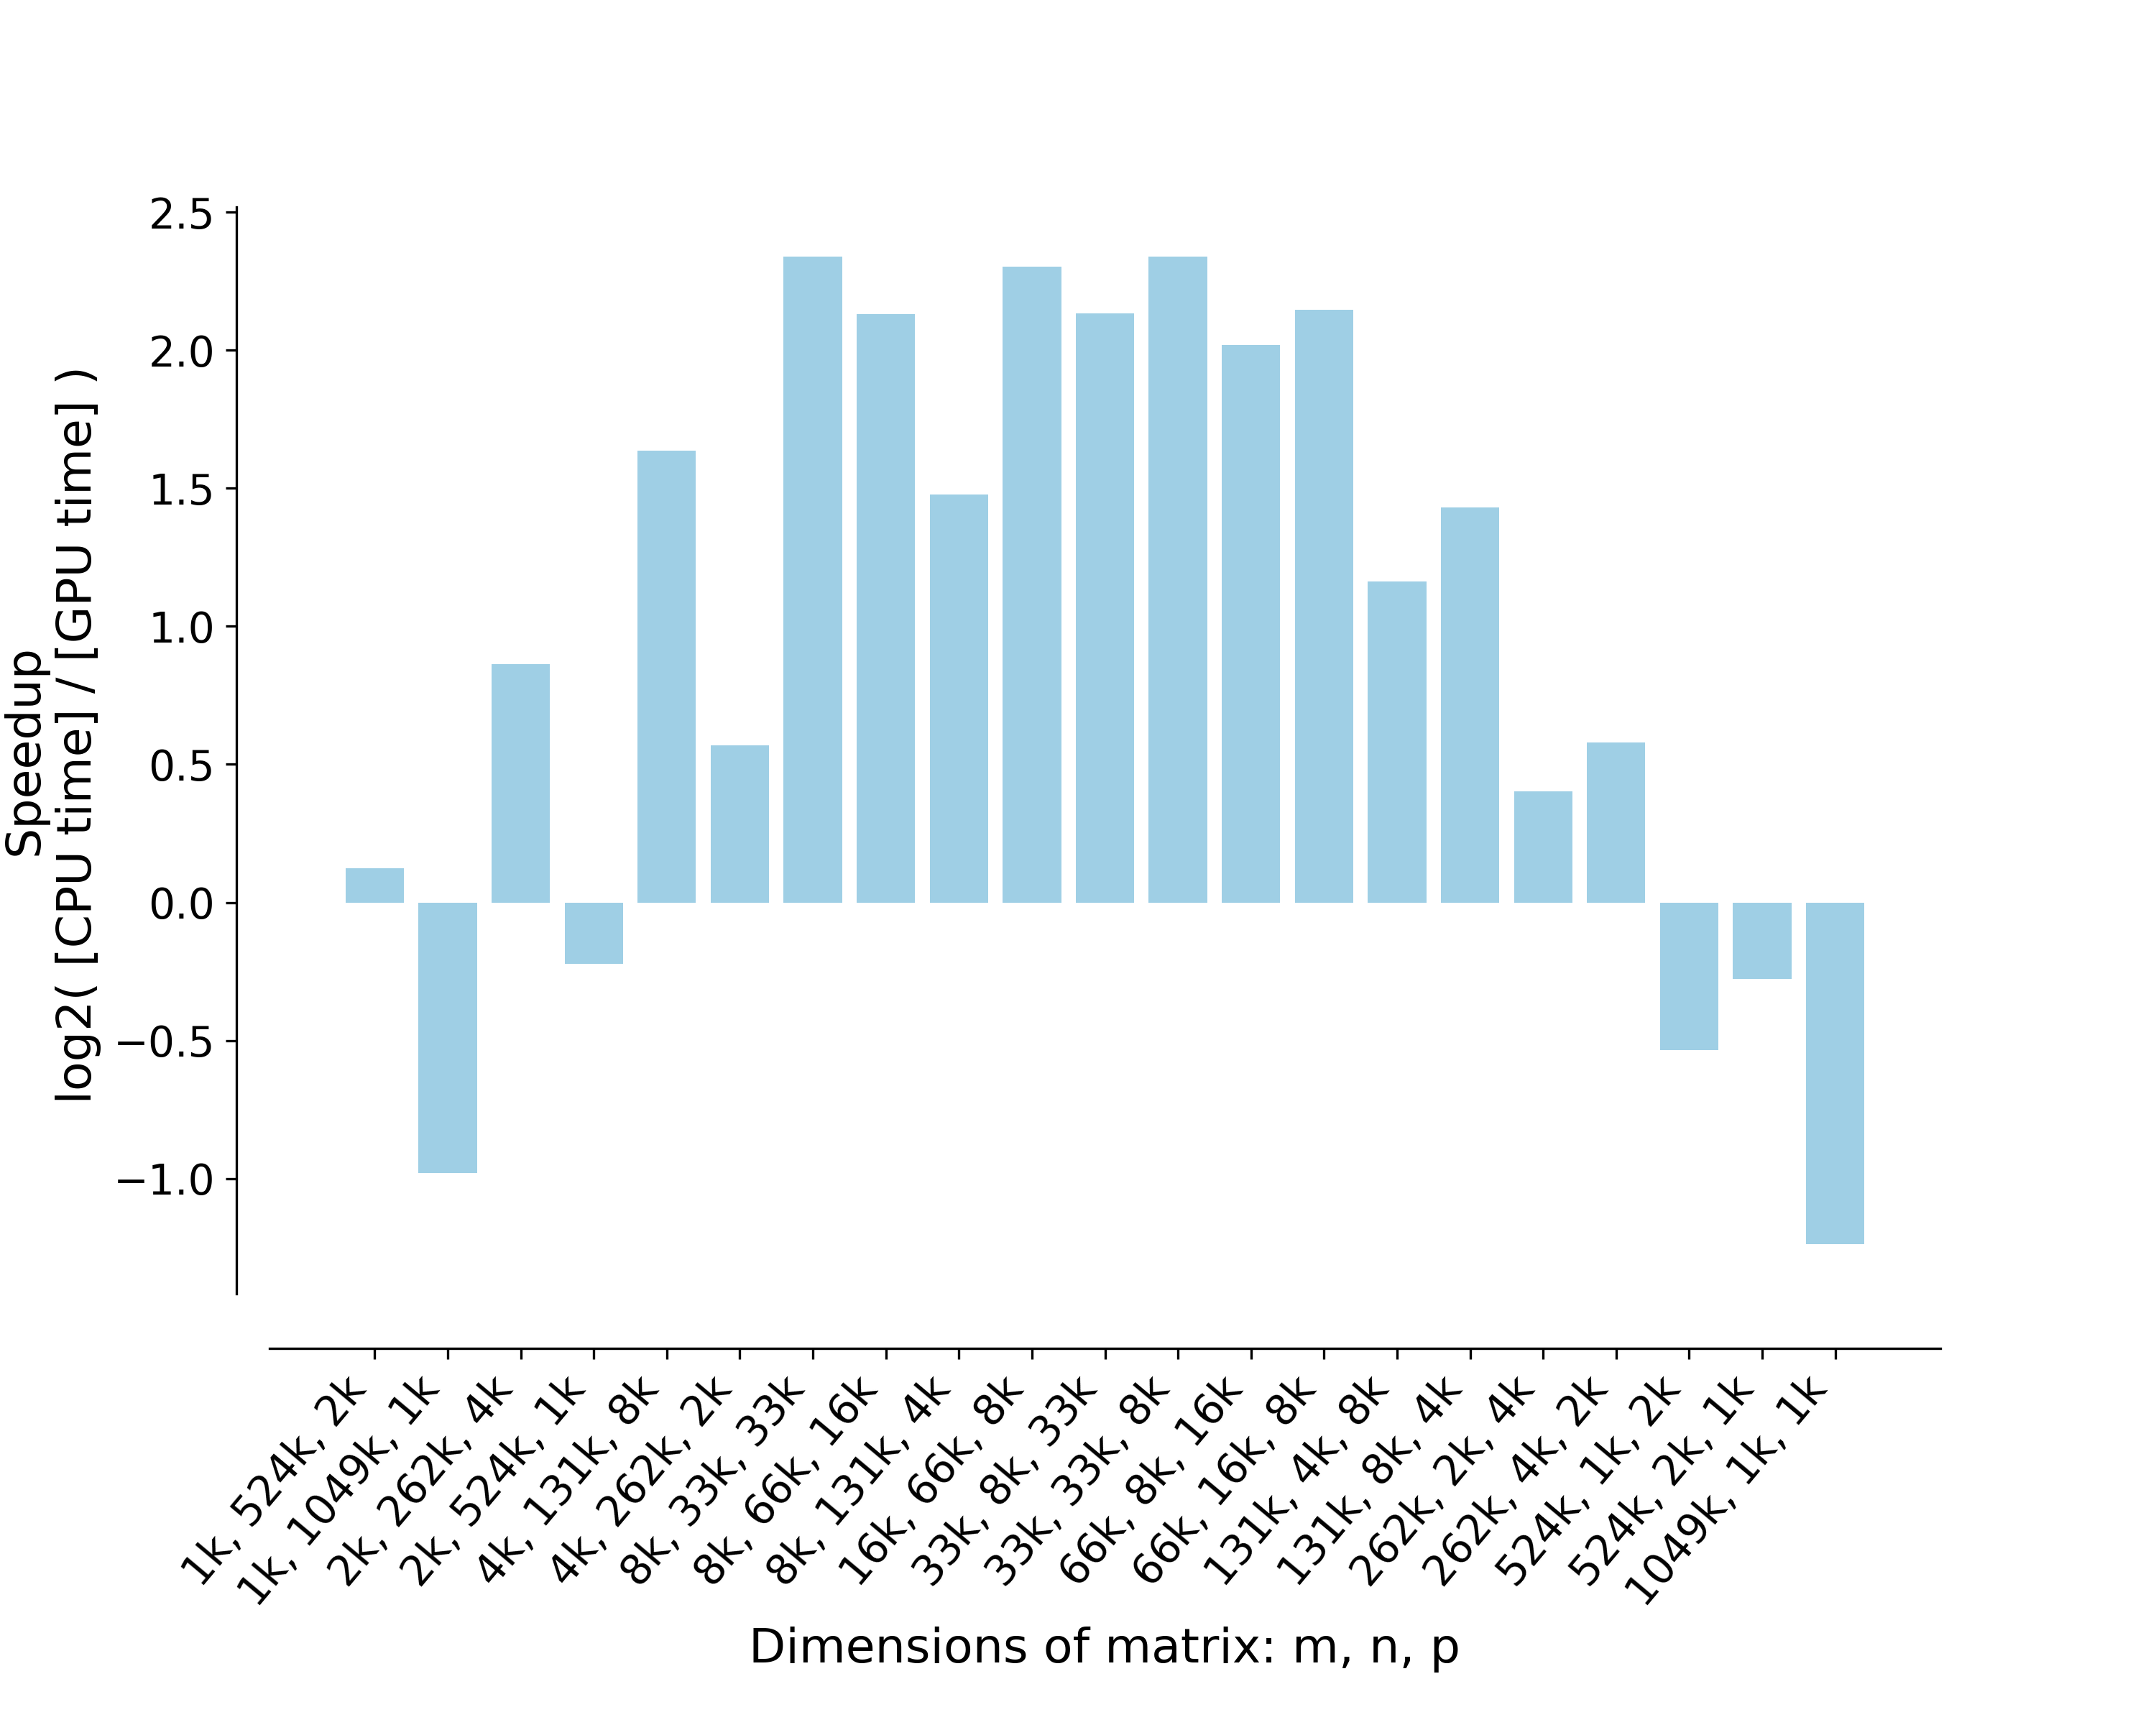
\includegraphics[scale = 0.4]{figs/speedup.png}
\end{figure} 


\subsection{Platform}
 \begin{itemize}
	\item CPU: Intel Xeon Gold 6148; 40 cores @ 2.40GHz, 192GB 
	\item GPU: Tesla V100-PCIE; 5120 Cores @ 1380 MHz, 16GB
\end{itemize}
Software: 
\begin{itemize}
	\item Programming environment: Julia; CentOS 7
	\item Libraries: CUDA v10.1 and cuBLAS; OpenBLAS
	\item Profilers: Julia Profiler Package; nvprof
\end{itemize}

%The results and discussion should not be repetitive. The results section should give a factual presentation of the data and all tables and figures should be referenced; the discussion should not summarize the results but provide an interpretation of the results, and should clearly delineate between the findings of the particular study and the possible impact of those findings in a larger context. Authors are encouraged to cite recent work relevant to their interpretations. Present and discuss results only once, not in both the Results and Discussion sections. It is sometimes acceptable to combine results and discussion. The text should be as succinct as possible. Heed Strunk and White's dictum: "Omit needless words!"


\section{Conclusion}





\subsection{Sample Table}

Table \ref{tab:shape-functions} shows an examplex table. 

\begin{table*}[htbp]
\renewcommand{\familydefault}{\sfdefault}\normalfont
\centering
\caption{\bf Students and their grades}
\begin{tableminipage}{\textwidth}
\begin{tabularx}{\textwidth}{XXXX}
\hline
\header Student & Grade\footnote{This is an example of a footnote in a table. Lowercase, superscript italic letters (a, b, c, etc.) are used by default. You can also use *, **, and *** to indicate conventional levels of statistical significance, explained below the table.} & Rank & Notes \\
\hline
Alice & 82\% & 1 & Performed very well.\\
Bob & 65\% & 3 & Not up to his usual standard.\\
Charlie & 73\% & 2 & A good attempt.\\
\hline
\end{tabularx}
  \label{tab:shape-functions}
\end{tableminipage}
\end{table*}


\bibliography{example-bibliography}

\end{document}
